% Generated by Sphinx.
\def\sphinxdocclass{report}
\documentclass[letterpaper,10pt,english]{sphinxmanual}
\usepackage[utf8]{inputenc}
\DeclareUnicodeCharacter{00A0}{\nobreakspace}
\usepackage{cmap}
\usepackage[T1]{fontenc}
\usepackage{babel}
\usepackage{times}
\usepackage[Bjarne]{fncychap}
\usepackage{longtable}
\usepackage{sphinx}
\usepackage{multirow}


\title{Proyecto ICARO, Documentación Documentation}
\date{February 17, 2016}
\release{0}
\author{Valentin Basel}
\newcommand{\sphinxlogo}{}
\renewcommand{\releasename}{Release}
\makeindex

\makeatletter
\def\PYG@reset{\let\PYG@it=\relax \let\PYG@bf=\relax%
    \let\PYG@ul=\relax \let\PYG@tc=\relax%
    \let\PYG@bc=\relax \let\PYG@ff=\relax}
\def\PYG@tok#1{\csname PYG@tok@#1\endcsname}
\def\PYG@toks#1+{\ifx\relax#1\empty\else%
    \PYG@tok{#1}\expandafter\PYG@toks\fi}
\def\PYG@do#1{\PYG@bc{\PYG@tc{\PYG@ul{%
    \PYG@it{\PYG@bf{\PYG@ff{#1}}}}}}}
\def\PYG#1#2{\PYG@reset\PYG@toks#1+\relax+\PYG@do{#2}}

\expandafter\def\csname PYG@tok@gd\endcsname{\def\PYG@tc##1{\textcolor[rgb]{0.63,0.00,0.00}{##1}}}
\expandafter\def\csname PYG@tok@gu\endcsname{\let\PYG@bf=\textbf\def\PYG@tc##1{\textcolor[rgb]{0.50,0.00,0.50}{##1}}}
\expandafter\def\csname PYG@tok@gt\endcsname{\def\PYG@tc##1{\textcolor[rgb]{0.00,0.27,0.87}{##1}}}
\expandafter\def\csname PYG@tok@gs\endcsname{\let\PYG@bf=\textbf}
\expandafter\def\csname PYG@tok@gr\endcsname{\def\PYG@tc##1{\textcolor[rgb]{1.00,0.00,0.00}{##1}}}
\expandafter\def\csname PYG@tok@cm\endcsname{\let\PYG@it=\textit\def\PYG@tc##1{\textcolor[rgb]{0.25,0.50,0.56}{##1}}}
\expandafter\def\csname PYG@tok@vg\endcsname{\def\PYG@tc##1{\textcolor[rgb]{0.73,0.38,0.84}{##1}}}
\expandafter\def\csname PYG@tok@m\endcsname{\def\PYG@tc##1{\textcolor[rgb]{0.13,0.50,0.31}{##1}}}
\expandafter\def\csname PYG@tok@mh\endcsname{\def\PYG@tc##1{\textcolor[rgb]{0.13,0.50,0.31}{##1}}}
\expandafter\def\csname PYG@tok@cs\endcsname{\def\PYG@tc##1{\textcolor[rgb]{0.25,0.50,0.56}{##1}}\def\PYG@bc##1{\setlength{\fboxsep}{0pt}\colorbox[rgb]{1.00,0.94,0.94}{\strut ##1}}}
\expandafter\def\csname PYG@tok@ge\endcsname{\let\PYG@it=\textit}
\expandafter\def\csname PYG@tok@vc\endcsname{\def\PYG@tc##1{\textcolor[rgb]{0.73,0.38,0.84}{##1}}}
\expandafter\def\csname PYG@tok@il\endcsname{\def\PYG@tc##1{\textcolor[rgb]{0.13,0.50,0.31}{##1}}}
\expandafter\def\csname PYG@tok@go\endcsname{\def\PYG@tc##1{\textcolor[rgb]{0.20,0.20,0.20}{##1}}}
\expandafter\def\csname PYG@tok@cp\endcsname{\def\PYG@tc##1{\textcolor[rgb]{0.00,0.44,0.13}{##1}}}
\expandafter\def\csname PYG@tok@gi\endcsname{\def\PYG@tc##1{\textcolor[rgb]{0.00,0.63,0.00}{##1}}}
\expandafter\def\csname PYG@tok@gh\endcsname{\let\PYG@bf=\textbf\def\PYG@tc##1{\textcolor[rgb]{0.00,0.00,0.50}{##1}}}
\expandafter\def\csname PYG@tok@ni\endcsname{\let\PYG@bf=\textbf\def\PYG@tc##1{\textcolor[rgb]{0.84,0.33,0.22}{##1}}}
\expandafter\def\csname PYG@tok@nl\endcsname{\let\PYG@bf=\textbf\def\PYG@tc##1{\textcolor[rgb]{0.00,0.13,0.44}{##1}}}
\expandafter\def\csname PYG@tok@nn\endcsname{\let\PYG@bf=\textbf\def\PYG@tc##1{\textcolor[rgb]{0.05,0.52,0.71}{##1}}}
\expandafter\def\csname PYG@tok@no\endcsname{\def\PYG@tc##1{\textcolor[rgb]{0.38,0.68,0.84}{##1}}}
\expandafter\def\csname PYG@tok@na\endcsname{\def\PYG@tc##1{\textcolor[rgb]{0.25,0.44,0.63}{##1}}}
\expandafter\def\csname PYG@tok@nb\endcsname{\def\PYG@tc##1{\textcolor[rgb]{0.00,0.44,0.13}{##1}}}
\expandafter\def\csname PYG@tok@nc\endcsname{\let\PYG@bf=\textbf\def\PYG@tc##1{\textcolor[rgb]{0.05,0.52,0.71}{##1}}}
\expandafter\def\csname PYG@tok@nd\endcsname{\let\PYG@bf=\textbf\def\PYG@tc##1{\textcolor[rgb]{0.33,0.33,0.33}{##1}}}
\expandafter\def\csname PYG@tok@ne\endcsname{\def\PYG@tc##1{\textcolor[rgb]{0.00,0.44,0.13}{##1}}}
\expandafter\def\csname PYG@tok@nf\endcsname{\def\PYG@tc##1{\textcolor[rgb]{0.02,0.16,0.49}{##1}}}
\expandafter\def\csname PYG@tok@si\endcsname{\let\PYG@it=\textit\def\PYG@tc##1{\textcolor[rgb]{0.44,0.63,0.82}{##1}}}
\expandafter\def\csname PYG@tok@s2\endcsname{\def\PYG@tc##1{\textcolor[rgb]{0.25,0.44,0.63}{##1}}}
\expandafter\def\csname PYG@tok@vi\endcsname{\def\PYG@tc##1{\textcolor[rgb]{0.73,0.38,0.84}{##1}}}
\expandafter\def\csname PYG@tok@nt\endcsname{\let\PYG@bf=\textbf\def\PYG@tc##1{\textcolor[rgb]{0.02,0.16,0.45}{##1}}}
\expandafter\def\csname PYG@tok@nv\endcsname{\def\PYG@tc##1{\textcolor[rgb]{0.73,0.38,0.84}{##1}}}
\expandafter\def\csname PYG@tok@s1\endcsname{\def\PYG@tc##1{\textcolor[rgb]{0.25,0.44,0.63}{##1}}}
\expandafter\def\csname PYG@tok@gp\endcsname{\let\PYG@bf=\textbf\def\PYG@tc##1{\textcolor[rgb]{0.78,0.36,0.04}{##1}}}
\expandafter\def\csname PYG@tok@sh\endcsname{\def\PYG@tc##1{\textcolor[rgb]{0.25,0.44,0.63}{##1}}}
\expandafter\def\csname PYG@tok@ow\endcsname{\let\PYG@bf=\textbf\def\PYG@tc##1{\textcolor[rgb]{0.00,0.44,0.13}{##1}}}
\expandafter\def\csname PYG@tok@sx\endcsname{\def\PYG@tc##1{\textcolor[rgb]{0.78,0.36,0.04}{##1}}}
\expandafter\def\csname PYG@tok@bp\endcsname{\def\PYG@tc##1{\textcolor[rgb]{0.00,0.44,0.13}{##1}}}
\expandafter\def\csname PYG@tok@c1\endcsname{\let\PYG@it=\textit\def\PYG@tc##1{\textcolor[rgb]{0.25,0.50,0.56}{##1}}}
\expandafter\def\csname PYG@tok@kc\endcsname{\let\PYG@bf=\textbf\def\PYG@tc##1{\textcolor[rgb]{0.00,0.44,0.13}{##1}}}
\expandafter\def\csname PYG@tok@c\endcsname{\let\PYG@it=\textit\def\PYG@tc##1{\textcolor[rgb]{0.25,0.50,0.56}{##1}}}
\expandafter\def\csname PYG@tok@mf\endcsname{\def\PYG@tc##1{\textcolor[rgb]{0.13,0.50,0.31}{##1}}}
\expandafter\def\csname PYG@tok@err\endcsname{\def\PYG@bc##1{\setlength{\fboxsep}{0pt}\fcolorbox[rgb]{1.00,0.00,0.00}{1,1,1}{\strut ##1}}}
\expandafter\def\csname PYG@tok@mb\endcsname{\def\PYG@tc##1{\textcolor[rgb]{0.13,0.50,0.31}{##1}}}
\expandafter\def\csname PYG@tok@ss\endcsname{\def\PYG@tc##1{\textcolor[rgb]{0.32,0.47,0.09}{##1}}}
\expandafter\def\csname PYG@tok@sr\endcsname{\def\PYG@tc##1{\textcolor[rgb]{0.14,0.33,0.53}{##1}}}
\expandafter\def\csname PYG@tok@mo\endcsname{\def\PYG@tc##1{\textcolor[rgb]{0.13,0.50,0.31}{##1}}}
\expandafter\def\csname PYG@tok@kd\endcsname{\let\PYG@bf=\textbf\def\PYG@tc##1{\textcolor[rgb]{0.00,0.44,0.13}{##1}}}
\expandafter\def\csname PYG@tok@mi\endcsname{\def\PYG@tc##1{\textcolor[rgb]{0.13,0.50,0.31}{##1}}}
\expandafter\def\csname PYG@tok@kn\endcsname{\let\PYG@bf=\textbf\def\PYG@tc##1{\textcolor[rgb]{0.00,0.44,0.13}{##1}}}
\expandafter\def\csname PYG@tok@o\endcsname{\def\PYG@tc##1{\textcolor[rgb]{0.40,0.40,0.40}{##1}}}
\expandafter\def\csname PYG@tok@kr\endcsname{\let\PYG@bf=\textbf\def\PYG@tc##1{\textcolor[rgb]{0.00,0.44,0.13}{##1}}}
\expandafter\def\csname PYG@tok@s\endcsname{\def\PYG@tc##1{\textcolor[rgb]{0.25,0.44,0.63}{##1}}}
\expandafter\def\csname PYG@tok@kp\endcsname{\def\PYG@tc##1{\textcolor[rgb]{0.00,0.44,0.13}{##1}}}
\expandafter\def\csname PYG@tok@w\endcsname{\def\PYG@tc##1{\textcolor[rgb]{0.73,0.73,0.73}{##1}}}
\expandafter\def\csname PYG@tok@kt\endcsname{\def\PYG@tc##1{\textcolor[rgb]{0.56,0.13,0.00}{##1}}}
\expandafter\def\csname PYG@tok@sc\endcsname{\def\PYG@tc##1{\textcolor[rgb]{0.25,0.44,0.63}{##1}}}
\expandafter\def\csname PYG@tok@sb\endcsname{\def\PYG@tc##1{\textcolor[rgb]{0.25,0.44,0.63}{##1}}}
\expandafter\def\csname PYG@tok@k\endcsname{\let\PYG@bf=\textbf\def\PYG@tc##1{\textcolor[rgb]{0.00,0.44,0.13}{##1}}}
\expandafter\def\csname PYG@tok@se\endcsname{\let\PYG@bf=\textbf\def\PYG@tc##1{\textcolor[rgb]{0.25,0.44,0.63}{##1}}}
\expandafter\def\csname PYG@tok@sd\endcsname{\let\PYG@it=\textit\def\PYG@tc##1{\textcolor[rgb]{0.25,0.44,0.63}{##1}}}

\def\PYGZbs{\char`\\}
\def\PYGZus{\char`\_}
\def\PYGZob{\char`\{}
\def\PYGZcb{\char`\}}
\def\PYGZca{\char`\^}
\def\PYGZam{\char`\&}
\def\PYGZlt{\char`\<}
\def\PYGZgt{\char`\>}
\def\PYGZsh{\char`\#}
\def\PYGZpc{\char`\%}
\def\PYGZdl{\char`\$}
\def\PYGZhy{\char`\-}
\def\PYGZsq{\char`\'}
\def\PYGZdq{\char`\"}
\def\PYGZti{\char`\~}
% for compatibility with earlier versions
\def\PYGZat{@}
\def\PYGZlb{[}
\def\PYGZrb{]}
\makeatother

\renewcommand\PYGZsq{\textquotesingle}

\begin{document}

\maketitle
\tableofcontents
\phantomsection\label{index::doc}


Contents:


\chapter{Introducción}
\label{introduccion:introduccion}\label{introduccion:welcome-to-proyecto-icaro-documentacion-s-documentation}\label{introduccion::doc}
La robótica pedagógica, dado su carácter multidisciplinario, permite el
abordaje de conocimientos variados como la electrónica, informática,
física y matemática mediante la construcción de un juguete-objeto
como puede ser un robot. El desarrollo de estos juguetes-objetos
implica una experiencia que contribuye a expandir la creatividad y el
pensamiento reflexivo y científico de los alumnos,
en relación a la formulación de hipótesis, la
experimentación y la elaboración de conclusiones, los cuales al
enfrentarse a un “problema” dado, aprenden a experimentar, diseñar y
resolver situaciones de carácter constructivista. En el proceso de
“pensar el robot” , se generan las condiciones de apropiación
del conocimiento por parte del alumno.
Se trata de otorgar a los alumnos un rol activo en sus aprendizajes,
colocándolos como diseñadores de sus propios proyectos y constructores
de conocimientos. El uso de software libre en el ámbito escolar,
permite tener control sobre las características del mismo,
permitiendo adaptarlo a las necesidades concretas del ámbito escolar
y las realidades socio-económicas de la institución, es neutro frente
a fabricantes (el alumno no es un “potencial cliente”) y todo el
material usado puede ponerse a disposición de otros docentes.


\section{software libre en la educación}
\label{introduccion:software-libre-en-la-educacion}
Antes de explicar que es el software libre,
necesitamos conocer algunos aspectos claves del diseño y
creación de cualquier programa, como el concepto de código fuente y
como afecta a nuestra libertad el echo de no poder tener acceso al mismo.

Una computadora es básicamente una máquina electrónica que recibe y
procesa datos para convertirlos en información útil, y esos datos
apenas son cadenas de ceros y/o unos. Por lo tanto una computadora
solo entiende código binario, Para hacer
un programa mas o menos complejo, necesitamos muchísimos “ceros y unos”,
lo que hace extremadamente complejo entender y programar en
“lenguaje de maquina”. Para ello se diseñaron “lenguajes” mas parecidos
a lo que un humano podría entender y mediante un software
compilador podíamos convertirlo en archivo binario que nuestra
computadora usa.

Podemos considerar al software como el Conjunto de programas,
instrucciones y reglas informáticas para ejecutar ciertas tareas en una
computadora por lo tanto es una parte central de una computadora
porque es el que controla todos los procesos electrónicos de la
misma. Para que una computadora haga algo, necesita un programa, y
este tuvo que ser creado escribiendo en un lenguaje especial las
instrucciones que dicho programa ejecutara, esto se conoce como
Código fuente.

El código fuente es un texto escrito en un lenguaje de programación
específico que puede ser leído por un programador, se puede considerar
como un conjunto de líneas de texto que son las instrucciones que
debe seguir la computadora. El código fuente esta escrito en primera
instancia por un programador en un formato de texto plano y para que
este archivo de texto pueda ser interpretado por una computadora,
tiene que ser procesado por un software llamado «compilador», el cual
en su definición más genérica, es un programa que toma como entrada un
texto escrito usando la semántica de cierto lenguaje y produce como
salida el texto de un programa en otro lenguaje. De esta manera podemos
obtener de un lenguaje natural similar al lenguaje humano, un archivo
en lenguaje de código maquina (código binario).

Para los programadores, leer el código maquina o código binario es una
actividad muy difícil, por eso para poder modificar o estudiar un
programa, se vuelve fundamental tener el código fuente original. A
causa de que muchas empresas desarrolladoras de software no permiten
conocer ni estudiar el código fuente de sus programas
(software privativo), en el año 1985 Richard Stallman y otros
entusiastas fundaron la Free Software Foundation con el objetivo de
promover el uso del software libre.

Cuando Hablamos de software libre, nos referimos a todo software que
por elección manifiesta de su autor, puede ser copiado,
estudiado, modificado, utilizado libremente con cualquier fin y
redistribuido con o sin cambios o mejoras. Para eso se definió 4
«libertades» básicas que tiene que tener todo software para poder ser
considerado de software libre:
\begin{enumerate}
\item {} 
La libertad de ejecutar el programa como se desea, con cualquier propósito (libertad 0).

\item {} 
La libertad de estudiar cómo funciona el programa, y cambiarlo para que haga lo que usted quiera (libertad 1). El acceso al código fuente es una condición necesaria para ello.

\item {} 
La libertad de redistribuir copias para ayudar a su prójimo (libertad 2).

\item {} 
La libertad de distribuir copias de sus versiones modificadas a terceros (libertad 3). Esto le permite ofrecer a toda la comunidad la oportunidad de beneficiarse de las modificaciones. El acceso al código fuente es una condición necesaria para ello.

\end{enumerate}


\section{hardware libre}
\label{introduccion:hardware-libre}
Menos difundido que el concepto de software libre, la idea del «hardware libre»
(o mas precisamente, Hardware de fuentes abierta) trata de hacer un paralelismo
entre las «cuatro libertades» del software libre, aplicadas a el diseño y protocolos de
un dispositivo fisico.

Decimos que el hardware es libre en tanto el diseño de fabricación y
el software con el que fueron echos esos diagramas, sean distribuidos con licencias libres.
Si bien, por su naturaleza física, un dispositivo (electrónico o mecánico) no puede ser
equiparado a un programa de software, y por lo tanto, no es correcto equiparar
las 4 libertades que se aplican al software libre a un objeto físico único,
si se puede especificar que su diseño, esquemas, planos y demás componentes no-fisicos,
tengan un tipo de licencia libre. De esta forma un diseño electrónico, puede ser estudiado,
modificado y distribuido bajo los principios de las licencias GNU GPL
(GNU General Public License) o similares.

Un PCB (Printed Circuit Board por sus siglas en ingles)
es es la superficie constituida por pistas de material conductor
sobre una base no conductora, se utiliza para interconectar los
distintos componentes electronicos
(resistensias electricas, capacitores, microcontroladores etc.) y
generar un circuito por donde circule la corriente electrica, esta
«tarjeta de circuito impreso» funciona como soporte fisico y esquema de
conexión electronico.

Cuando se diseña un PCB, generalmente se necesitan 3 diagramas ,
el plano esquematico, el diseño del PCB y los ficheros de fabricación
archivos (GERBER). Con esa información podemos fabricar nuestra propia
versón de la plaqueta donde van soldados los componentes electronicos.

La ventaja del hardware libre es que permite adaptar nuestro diseño a
las distintas realidades locales donde se implementara la fabricación
de dicho dispositivo. De esta forma permite tener cierta independencia
de un fabricante en particular, y hasta permitir la fabricación a
pequeña escala (si el diseño asi lo permite), ademas de fomantar la
industria nacional y pequeñas PYMES o cooperativas que fabriquen el
hardware, aprovechando una comunidad de usuarios que
documentan y dan soporte al mismo.

Un caso muy significativo de la movida del hardware libre, son las
«impresoras 3d», dispositivo mecanico que permite fabricar componentes
de 3 dimensiones mediante superponer capas de plastico derretido en una
plataforma (usando distintos tipos de plasticos y hasta materiales
como cemento o metales fundidos en maquinas mas experimentales)
para lograr mediante la adicion sucesiva de capas de material, un
objecto tri dimensional con cierta consistencia y duresa.

Si bien la tecnologia de fabricación automatizada de piezas mecanicas
existe desde hace mucho (los sistemas CNC o control numérico por
computadora por ejemplo), el proyecto REPRAP se propuso fabricar una
maquina-herramienta de bajo costo capas de «auto replicarse» fabricando
las piezas para otras maquinas iguales. los creadores del proyecto
visionan la posibilidad de distribuir a bajo costo máquinas RepRap a
personas y comunidades, permitiéndoles crear (o descargar de Internet)
productos y objetos complejos sin la necesidad de maquinaria
industrial costosa. En ese sentido la idea del proyecto es poder
diseñar una impresora que pueda ser facilmente fabricada
por otras personas, sin necesidad de componentes industriales o
maquinaria especial para su fabricación. Obviamente, implica
una desición de compromiso entre cierta calidad de componentes y la
facilidad de obtenerlos a pequeña escala, ademas de los
conocimientos minimos necesarios para poder fabricar una impresora
(desde conocimientos sobre electronica a cuestines mecanicas
y cierta habilidad manual), por eso, comenzo a proliferar pequeñas
compañias o micro emprendimientos de personas que fabrican y
venden impresoras 3d basadas en los modelos de reprap (prusa I2 o
tambien prusa I3). De esta forma un proyecto global que nace
gracias a internet, genera trabajo para comunidades en distintas
partes del mundo.

En cierta forma, se podria decir que el hardware libre rescata la
cultura del «hagalo usted mismo»
(o DIY por sus siglas en ingles), aunque hay proyectos comerciales muy
exitosos (como el caso de ARDUINO® y RASPBERRY PI®)
que son de carácter mas industrial y que sin embargo aprovechan
la ventaja de liberar sus diseños para contar con ua gran
scomunidad de usuarios que utilizan su hardware y crean documentación o
tutoriales a traves de internet.


\chapter{placa robotica \emph{np07}}
\label{np07:placa-robotica-pcb}\label{np07::doc}
El hardware \emph{np07}


\section{caracteristicas tecnicas}
\label{np07:caracteristicas-tecnicas}
bla


\section{listado de componentes}
\label{np07:listado-de-componentes}
\begin{tabulary}{\linewidth}{|L|L|L|L|}
\hline
\textsf{\relax 
Cantidad
} & \textsf{\relax 
Componente
} & \textsf{\relax 
Ubicación
} & \textsf{\relax 
imagen
}\\
\hline
11
 & 
Resistencias 470 Ohm - 1/4W
 & 
R1 R2 R3 R4 R5 R6 R7 R8 R9 R12 R17
 & 
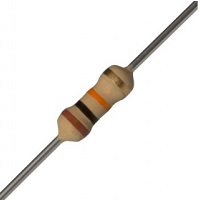
\includegraphics[width=40pt,height=40pt]{resistencia-10k.jpg}
\\

5
 & 
Resistencias 10k Ohm - 1/4W
 & 
R11 R13 R14 R15 R16
 & 
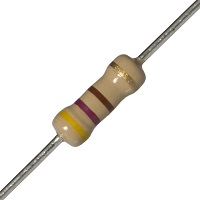
\includegraphics[width=40pt,height=40pt]{resistencia-470.jpg}
\\

2
 & 
Capacitores Cerámicos 22pF
 & 
C2 C3
 & 
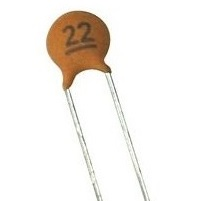
\includegraphics[width=40pt,height=40pt]{capacitor-22pf.jpg}
\\

5
 & 
Capacitores Cerámicos 0.1uF
 & 
C9 C10 C11 (C12 C13)*
 & 
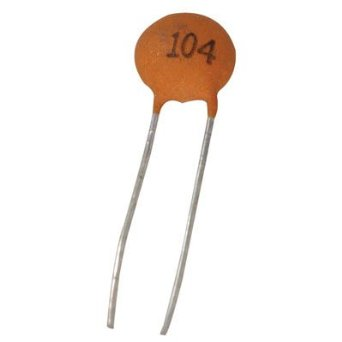
\includegraphics[width=40pt,height=40pt]{capacitor-01uf.jpg}
\\

1
 & 
Capacitor Cerámico 220nF
 & 
C1
 & 
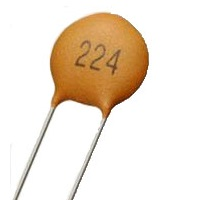
\includegraphics[width=40pt,height=40pt]{capacitor-220nf.jpg}
\\

1
 & 
Capacitor Electrol. 10uF 16V
 & 
C5
 & 
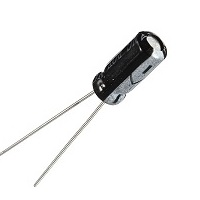
\includegraphics[width=40pt,height=40pt]{capacitorelectrolitico.jpg}
\\

4
 & 
Capacitor Electrol. 100uF
 & 
C4 C6 C7 C8
 & 
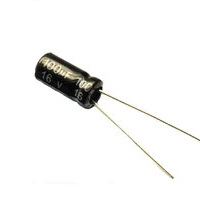
\includegraphics[width=40pt,height=40pt]{capacitor-100uf.jpg}
\\

3
 & 
Diodos 1N4007
 & 
D9 D12 D14
 & 
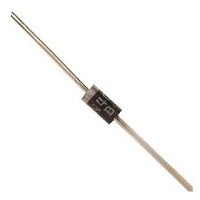
\includegraphics[width=40pt,height=40pt]{diodo-1n4007.jpg}
\\

11
 & 
Leds difusos 5mm
 & 
D1 D2 D3 D4 D5 D6 D7 D8 D10 D11 D12
 & 
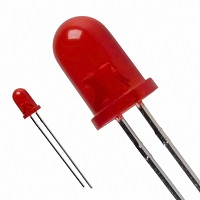
\includegraphics[width=40pt,height=40pt]{led-difusos-5mm.jpg}
\\

1
 & 
Conector USB hembra Tipo B
 & 
J1
 & 
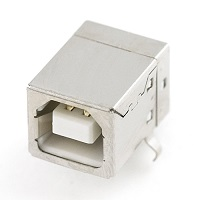
\includegraphics[width=40pt,height=40pt]{conector-usb-b.jpg}
\\
\hline\end{tabulary}


\begin{tabulary}{\linewidth}{|L|L|L|L|}
\hline
\textsf{\relax 
Cantidad
} & \textsf{\relax 
Componente
} & \textsf{\relax 
Ubicación
} & \textsf{\relax 
imagen
}\\
\hline
1
 & 
Push Button (Soft Touch)
 & 
SW2
 & 
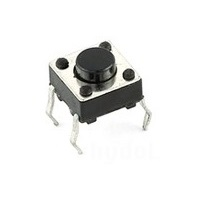
\includegraphics[width=40pt,height=40pt]{pushbutton.jpg}
\\

1
 & 
Regulador de Voltaje LM7805
 & 
U4
 & 
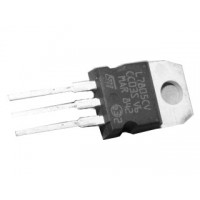
\includegraphics[width=40pt,height=40pt]{lm7805.jpg}
\\

1
 & 
Regulador de Voltaje 78L05
 & 
U5
 & 
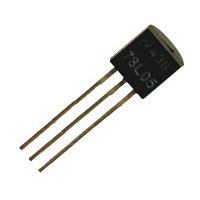
\includegraphics[width=40pt,height=40pt]{78L05.jpg}
\\

7
 & 
Borneras Dobles
 & 
P8 P9 P10 P11 P12 P13 P14
 & 
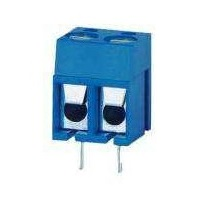
\includegraphics[width=40pt,height=40pt]{bornera.jpg}
\\

1
 & 
Zócalo de 8x2 Pines
 & 
U3
 & 
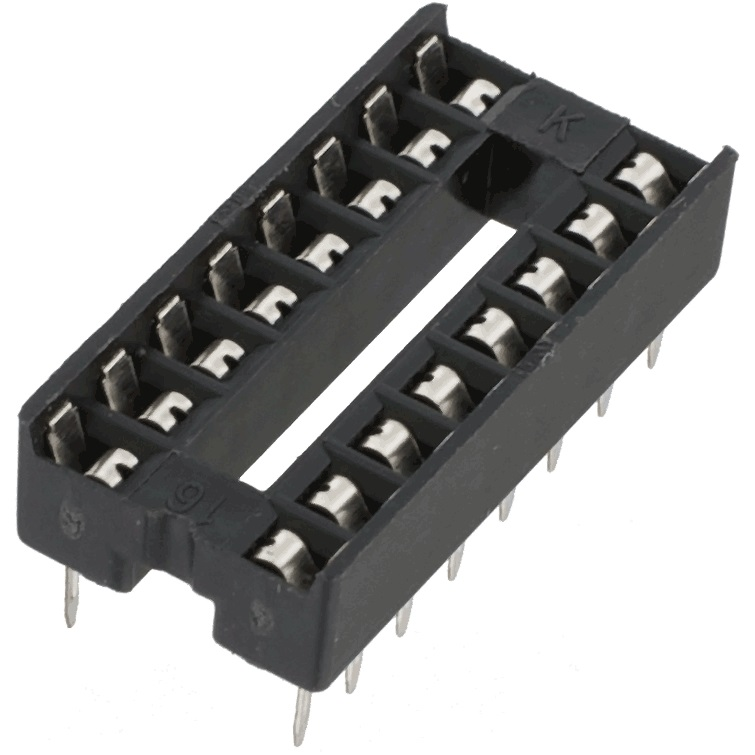
\includegraphics[width=40pt,height=40pt]{zocalo-8.jpg}
\\

1
 & 
Zócalo de 20x2 Pines
 & 
U2
 & 
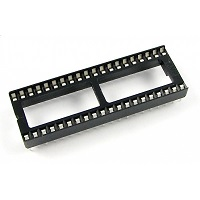
\includegraphics[width=40pt,height=40pt]{zocalo-20.jpg}
\\

1
 & 
Zócalo de 9x2 Pines
 & 
P6
 & 
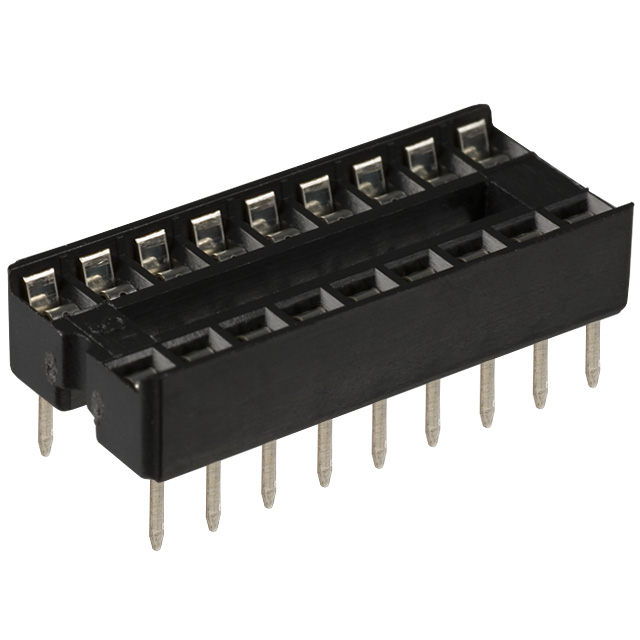
\includegraphics[width=40pt,height=40pt]{zocalo-9.jpg}
\\

1
 & 
Cristal de 20Mhz
 & 
X1
 & 
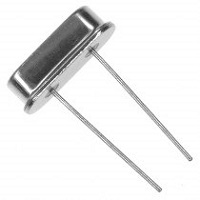
\includegraphics[width=40pt,height=40pt]{cristal-20mhz.jpg}
\\

2
 & 
Tira Postes Macho de 40 Pines
 & 
K2 K3 K4 K5 K6 SW1 SW3 K1 K8 P4
 & 
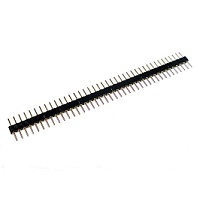
\includegraphics[width=40pt,height=40pt]{pinesmacho.jpg}
\\

1
 & 
Tira de Postes Hembra de 40 Pines
 & 
P1 P7 P5 P15 P16 P17 P18
 & 
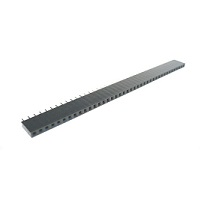
\includegraphics[width=40pt,height=40pt]{pineshembra.jpg}
\\

1
 & 
Driver L293D (Puente H)
 & 
U3
 & 
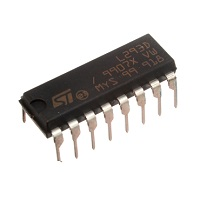
\includegraphics[width=40pt,height=40pt]{L293D.jpg}
\\

1
 & 
Integrado ULN2803
 & 
P6
 & 
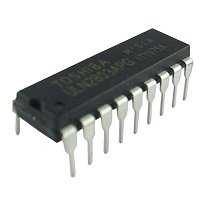
\includegraphics[width=40pt,height=40pt]{uln2803.jpg}
\\

1
 & 
Microcontrolador PIC18F4550
 & 
U2
 & 
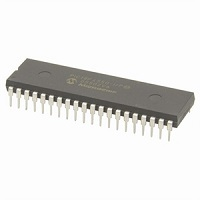
\includegraphics[width=40pt,height=40pt]{pic18f4550.jpg}
\\

4
 & 
jumper
 & 
SW1 SW3 K1 K8
 & 
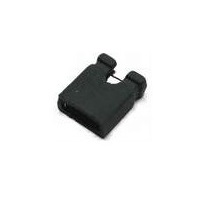
\includegraphics[width=40pt,height=40pt]{Jumper.jpg}
\\
\hline\end{tabulary}



\section{herramientas}
\label{np07:herramientas}
Las herramientas que necesitamos para armar una placa robotica \emph{np07}
son faciles de conseguir y muy comunes para cualquier
hobbista de la electronica.
\begin{figure}[htbp]
\centering
\capstart

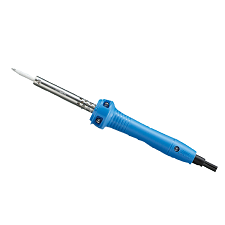
\includegraphics[width=300pt]{soldador.png}
\caption{Soldador}\end{figure}

Un soldador eléctrico o de estaño, también conocido como cautín, es
una herramienta eléctrica usada para soldar. Funciona convirtiendo
la energía eléctrica en calor, que a su vez provoca
la fusión del material utilizado en la soldadura, como por
ejemplo el estaño.
\newpage\begin{figure}[htbp]
\centering
\capstart

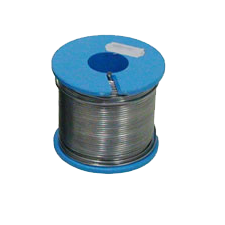
\includegraphics[width=300pt]{estanio.png}
\caption{Estaño}\end{figure}

El estaño que se utiliza en electrónica tiene alma de resina con el fin
de facilitar la soldadura. Para garantizar una buena soldadura es
necesario que tanto el estaño como el elemento a soldar alcancen una
temperatura determinada, si esta temperatura no se alcanza se produce
el fenómeno denominado soldadura fría. La temperatura de fusión
depende de la aleación utilizada, cuyo componente principal es
el estaño y suele estar comprendida entre unos 200 a 400 ºC.

En realidad, el término ``estaño'' se emplea de forma impropia
porque no se trata de estaño sólo, sino de una aleación de este metal
con plomo, generalmente con una proporción respectiva
del 60\% y del 40\%, que resulta ser la más indicada para
las soldaduras en Electrónica.

Para realizar una buena soldadura, además del soldador
y de la aleación descrita, se necesita una sustancia adicional,
llamada pasta de soldar, cuya misión es la de facilitar la distribución
uniforme del estaño sobre las superficies a unir y evitando, al mismo
tiempo, la oxidación producida por la temperatura demasiado elevada
del soldador. La composición de esta pasta es a base de colofonia
(normalmente llamada ``resina'') y que en el caso del estaño que
utilizaremos, está contenida dentro de las cavidades del hilo,
en una proporción del 2\textasciitilde{}2.5\%.
\newpage\begin{figure}[htbp]
\centering
\capstart

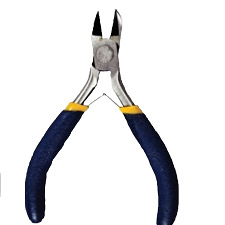
\includegraphics[width=300pt]{alicate.png}
\caption{alicate para electronica}\end{figure}

Un pequeño alicate, para poder cortar el excedente de material (estaño,
alambres de las resistensias por ejmplo).
\newpage\begin{figure}[htbp]
\centering
\capstart

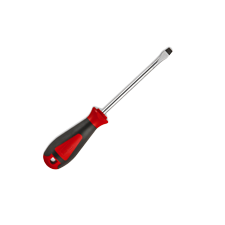
\includegraphics[width=300pt]{destornillador.png}
\caption{destornillador plano pequeño}\end{figure}

Nos sirve para ajustar las borneras y para hacer palanca para sacar un
integrado que hayamos puesto en un zocalo.
\newpage\begin{figure}[htbp]
\centering
\capstart

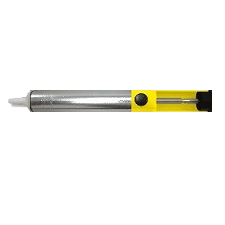
\includegraphics[width=300pt]{desoldador.png}
\caption{desoldador de estaño}\end{figure}

El desoldador de estaño, nos permite sacar el estaño que hayamos puesto
de mas o para remplazar algun componente efectuoso de la placa robotica \emph{np07}
\newpage

\section{fabricacion}
\label{np07:fabricacion}
A continución veremos el paso a paso del armado de la placa \emph{np07}.


\subsection{paso 0}
\label{np07:paso-0}\begin{figure}[htbp]
\centering
\capstart

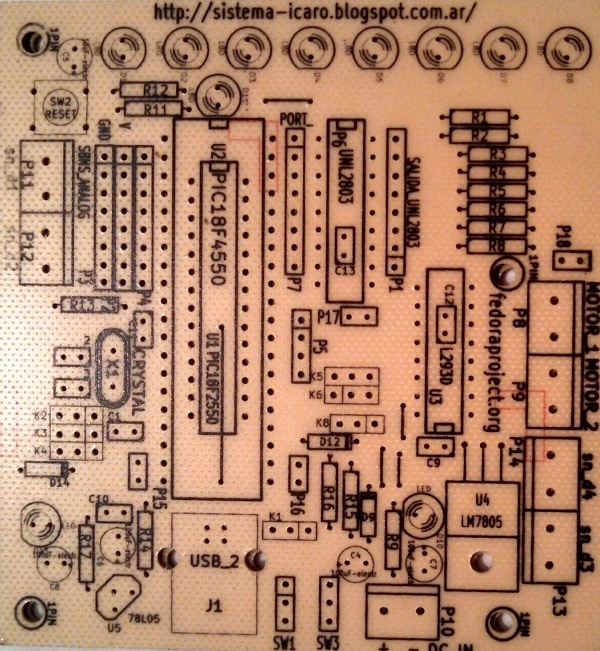
\includegraphics[width=300pt]{0b.jpg}
\caption{Vista de la Placa}\end{figure}
\newpage

\subsection{paso 1}
\label{np07:paso-1}\begin{figure}[htbp]
\centering
\capstart

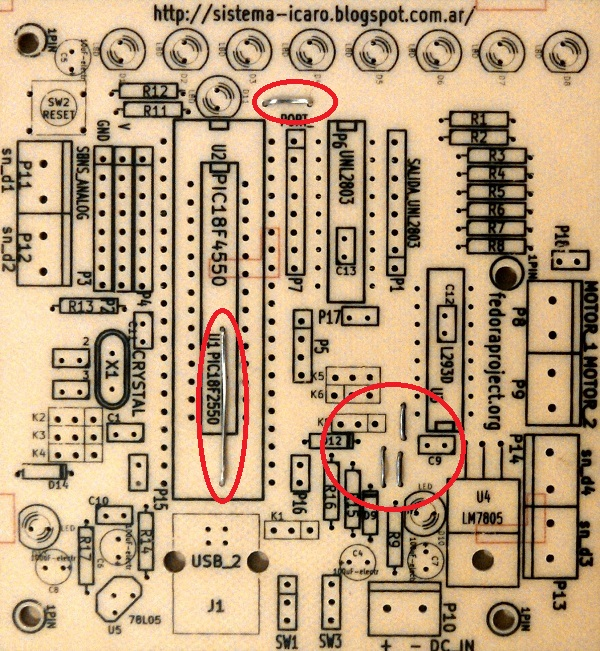
\includegraphics[width=300pt]{1b.jpg}
\caption{Colocar 5 Puentes}\end{figure}
\newpage

\subsection{paso 2}
\label{np07:paso-2}\begin{figure}[htbp]
\centering
\capstart

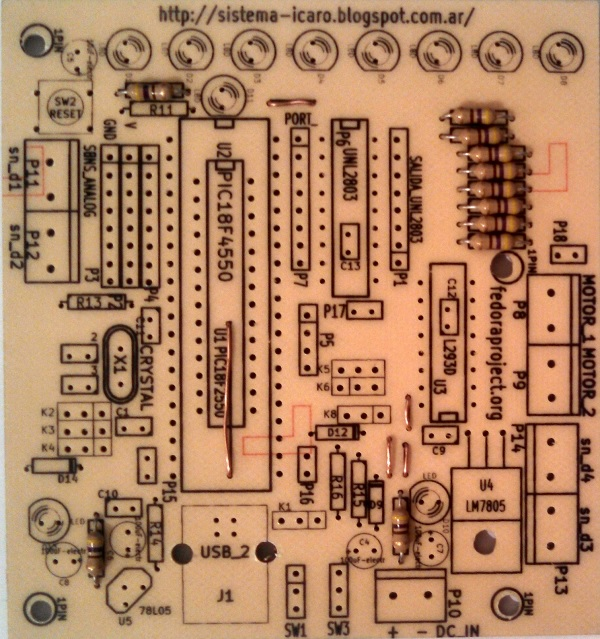
\includegraphics[width=300pt]{2b.jpg}
\caption{Resistencias de 470 Ohm}\end{figure}
\newpage

\subsection{paso 3}
\label{np07:paso-3}\begin{figure}[htbp]
\centering
\capstart

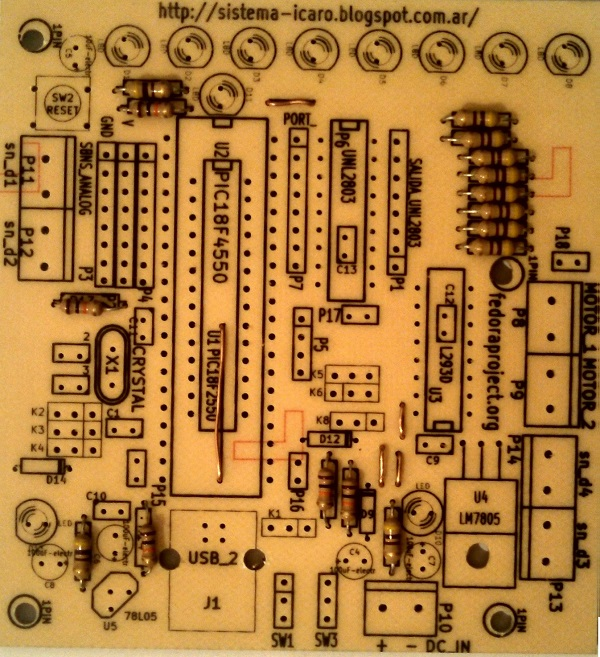
\includegraphics[width=300pt]{3b.jpg}
\caption{Resistencias de 10K Ohm}\end{figure}
\newpage

\subsection{paso 4}
\label{np07:paso-4}\begin{figure}[htbp]
\centering
\capstart

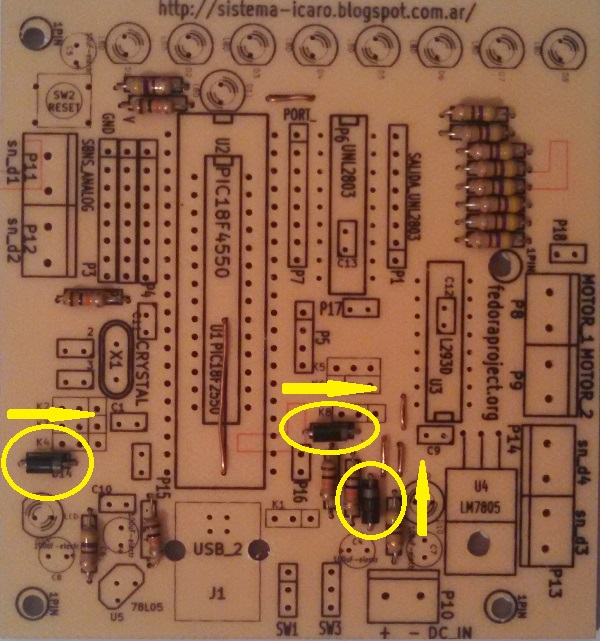
\includegraphics[width=300pt]{4b.jpg}
\caption{Diodos 1N4007}\end{figure}
\newpage

\subsection{paso 5}
\label{np07:paso-5}\begin{figure}[htbp]
\centering
\capstart

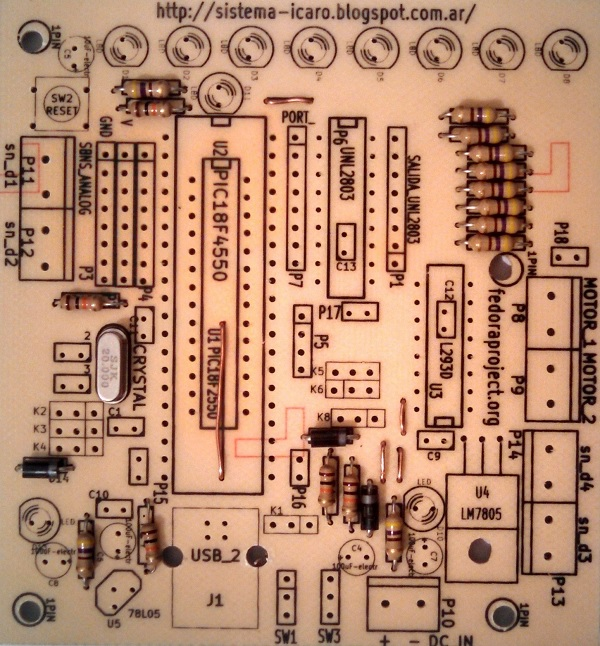
\includegraphics[width=300pt]{5b.jpg}
\caption{Cristal de 20MHz}\end{figure}
\newpage

\subsection{paso 6}
\label{np07:paso-6}\begin{figure}[htbp]
\centering
\capstart

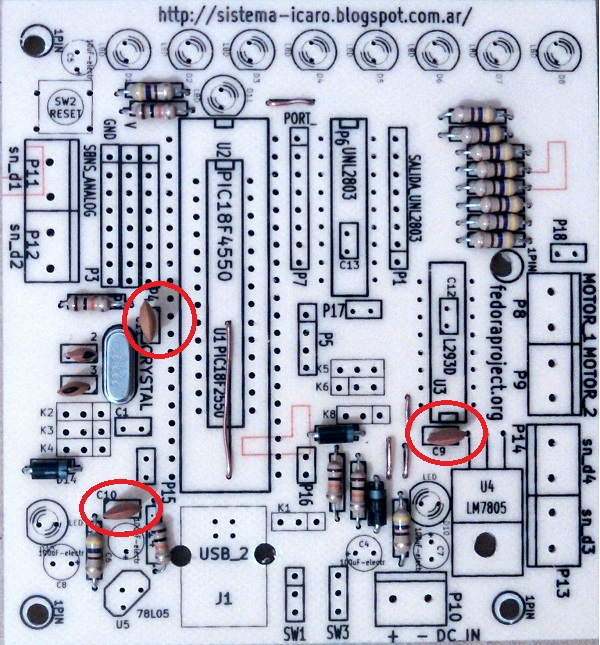
\includegraphics[width=300pt]{6b.jpg}
\caption{Capacitores Cerámicos 0,1uF}\end{figure}
\newpage

\subsection{paso 7}
\label{np07:paso-7}\begin{figure}[htbp]
\centering
\capstart

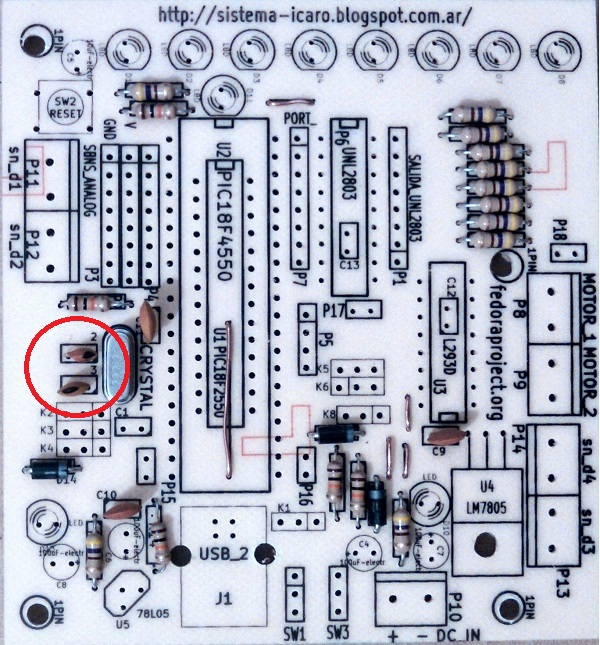
\includegraphics[width=300pt]{7b.jpg}
\caption{Capacitores Cerámicos 22pF}\end{figure}
\newpage

\subsection{paso 8}
\label{np07:paso-8}\begin{figure}[htbp]
\centering
\capstart

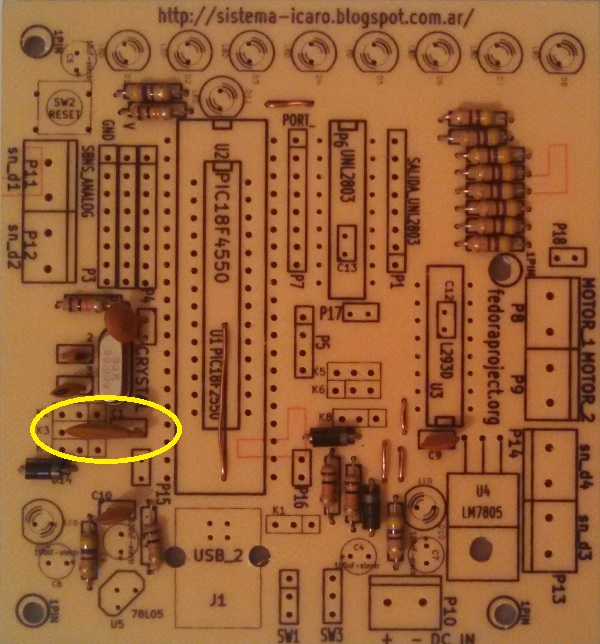
\includegraphics[width=300pt]{8b.jpg}
\caption{Capacitor Cerámico 220nF}\end{figure}
\newpage

\subsection{paso 9}
\label{np07:paso-9}\begin{figure}[htbp]
\centering
\capstart

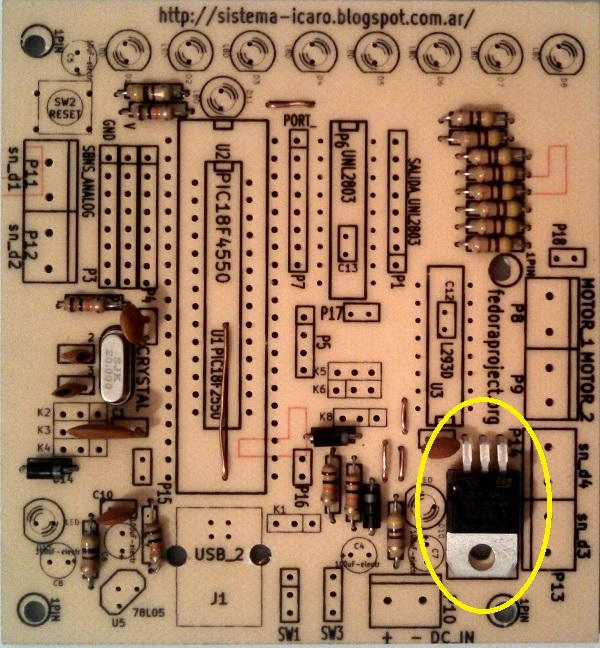
\includegraphics[width=300pt]{9b.jpg}
\caption{Regulador LM7805}\end{figure}
\newpage

\subsection{paso 10}
\label{np07:paso-10}\begin{figure}[htbp]
\centering
\capstart

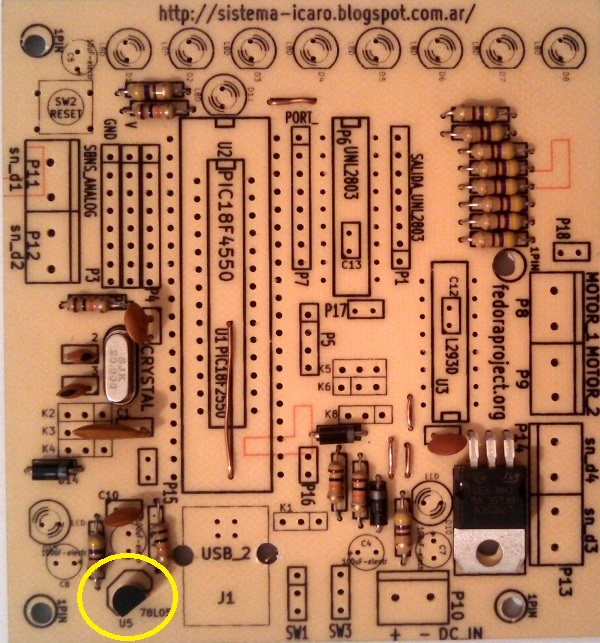
\includegraphics[width=300pt]{10b.jpg}
\caption{Regulador 78L05}\end{figure}
\newpage

\subsection{paso 11}
\label{np07:paso-11}\begin{figure}[htbp]
\centering
\capstart

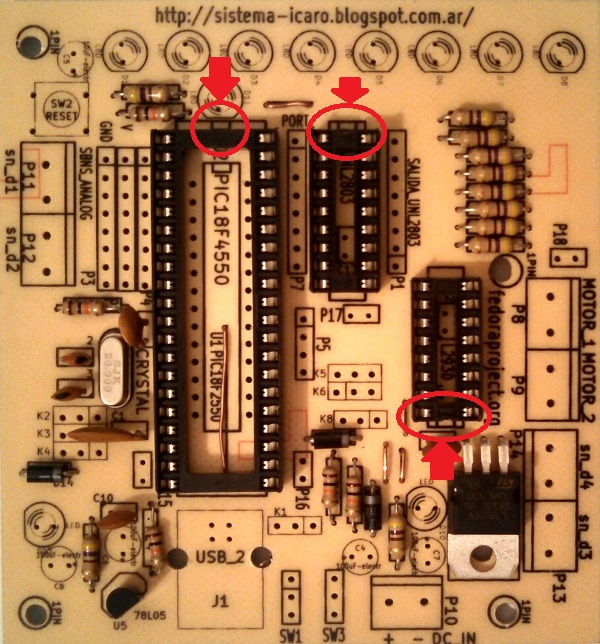
\includegraphics[width=300pt]{11b.jpg}
\caption{Colocar Zócalos}\end{figure}
\newpage

\subsection{paso 12}
\label{np07:paso-12}\begin{figure}[htbp]
\centering
\capstart

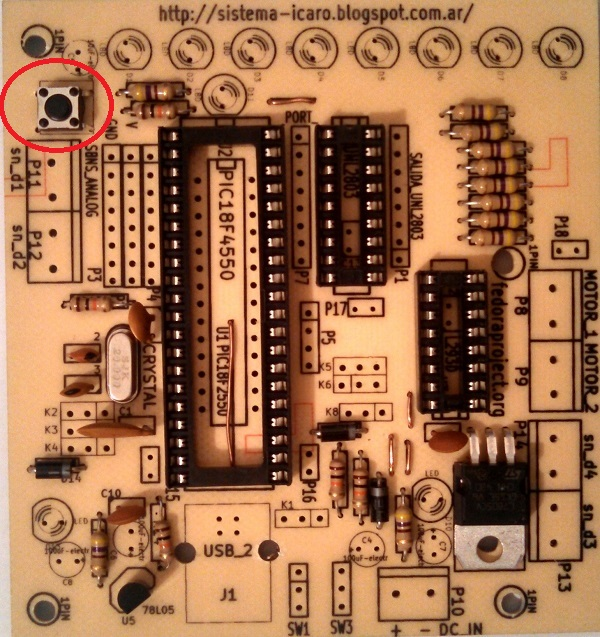
\includegraphics[width=300pt]{12b.jpg}
\caption{Push Button}\end{figure}
\newpage

\subsection{paso 13}
\label{np07:paso-13}\begin{figure}[htbp]
\centering
\capstart

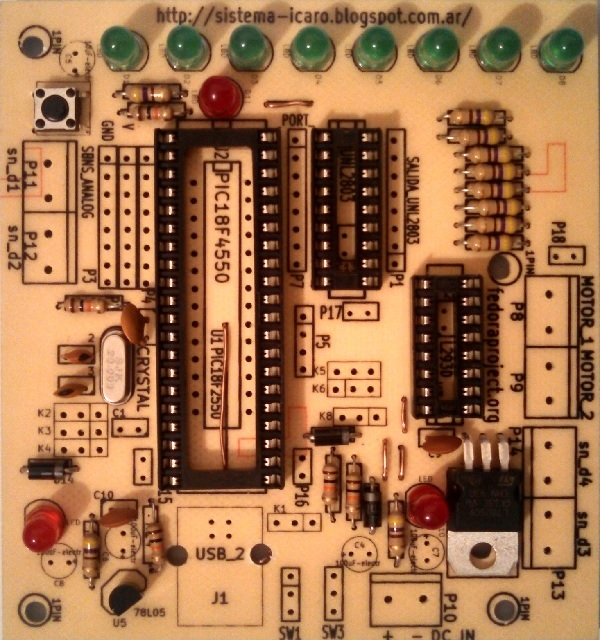
\includegraphics[width=300pt]{13b.jpg}
\caption{Colocar LEDS}\end{figure}
\newpage

\subsection{paso 14}
\label{np07:paso-14}\begin{figure}[htbp]
\centering
\capstart

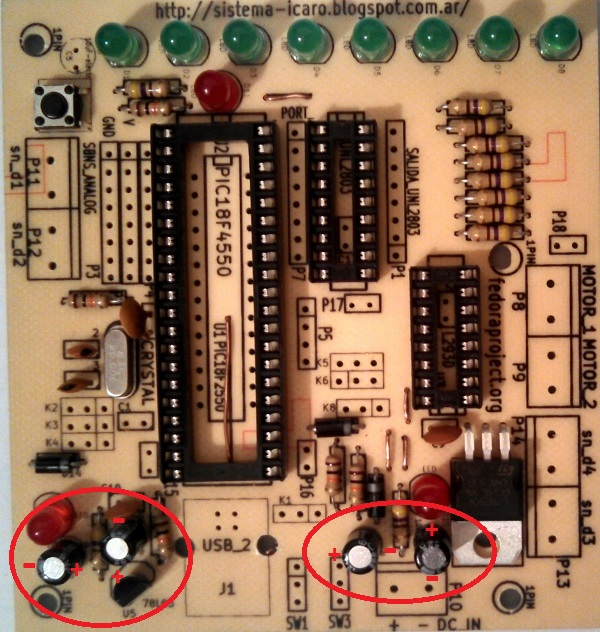
\includegraphics[width=300pt]{14b.jpg}
\caption{Capacitores Electrolíticos 100uF}\end{figure}
\newpage

\subsection{paso 15}
\label{np07:paso-15}\begin{figure}[htbp]
\centering
\capstart

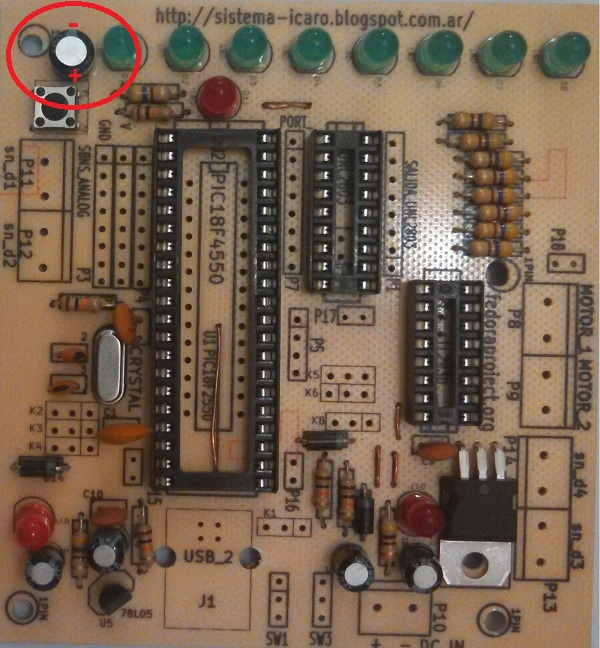
\includegraphics[width=300pt]{15b.jpg}
\caption{Capacitor Electrolítico 10uF}\end{figure}
\newpage

\subsection{paso 16}
\label{np07:paso-16}\begin{figure}[htbp]
\centering
\capstart

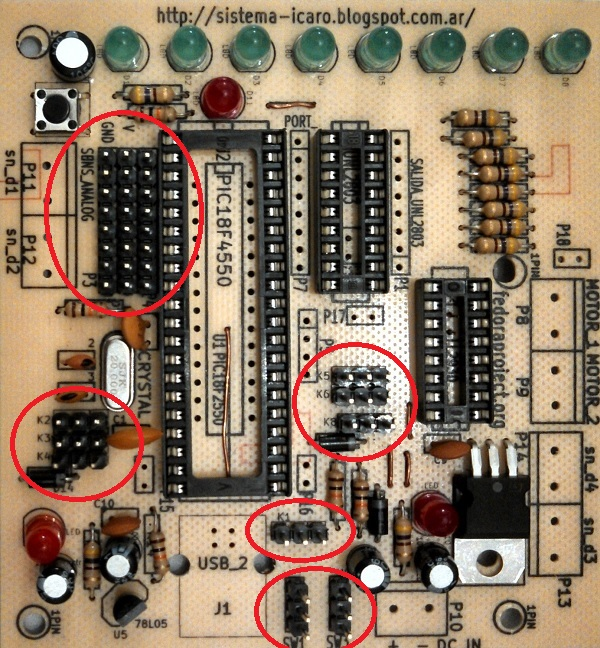
\includegraphics[width=300pt]{16b.jpg}
\caption{Postes Macho}\end{figure}
\newpage

\subsection{paso 17}
\label{np07:paso-17}\begin{figure}[htbp]
\centering
\capstart

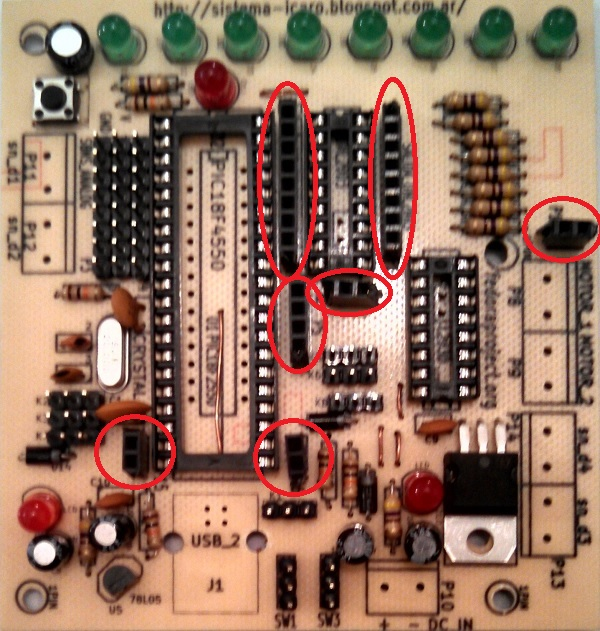
\includegraphics[width=300pt]{17b.jpg}
\caption{Postes Hembra}\end{figure}
\newpage

\subsection{paso 18}
\label{np07:paso-18}\begin{figure}[htbp]
\centering
\capstart

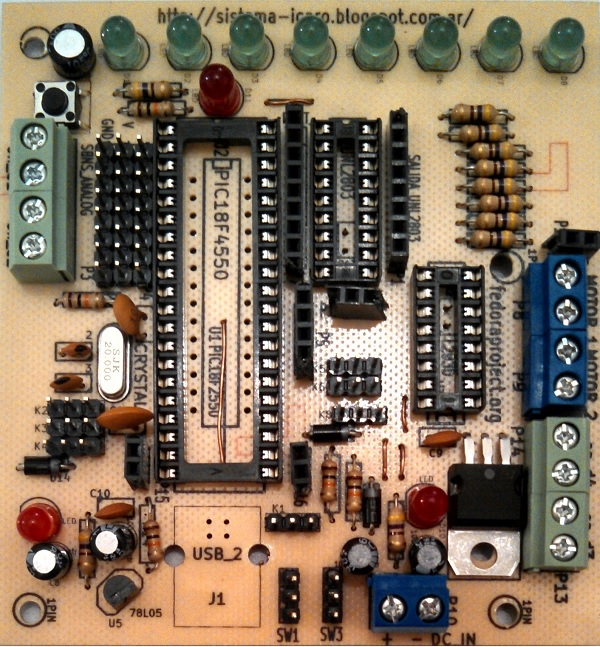
\includegraphics[width=300pt]{18b.jpg}
\caption{Borneras}\end{figure}
\newpage

\subsection{paso 19}
\label{np07:paso-19}\begin{figure}[htbp]
\centering
\capstart

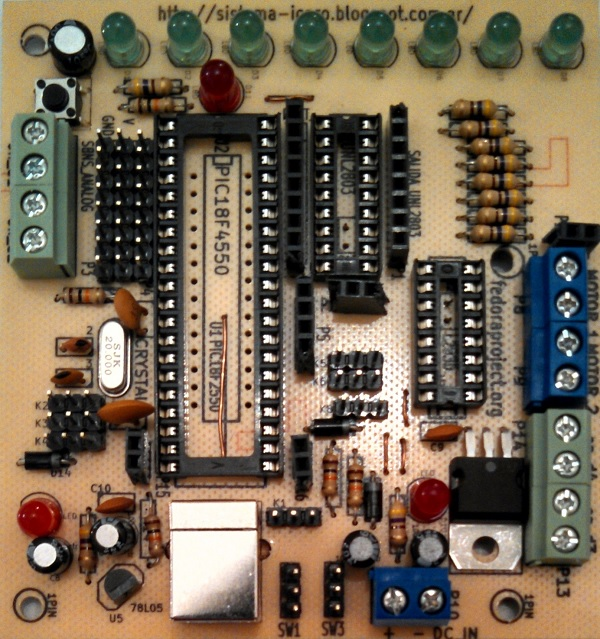
\includegraphics[width=300pt]{19b.jpg}
\caption{Conector USB hembra B}\end{figure}
\newpage

\subsection{paso 20}
\label{np07:paso-20}\begin{figure}[htbp]
\centering
\capstart

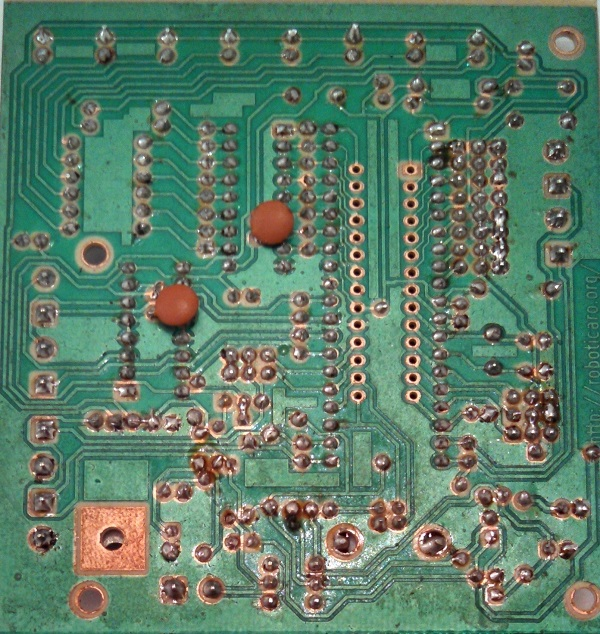
\includegraphics[width=300pt]{20b.jpg}
\caption{Capacitores Cerámicos 0,1uF}\end{figure}
\newpage

\chapter{icaro-bloques}
\label{icaro_bloques:icaro-bloques}\label{icaro_bloques::doc}
bla


\section{barra de herramientas}
\label{icaro_bloques:barra-de-herramientas}
bla


\section{barra de componentes}
\label{icaro_bloques:barra-de-componentes}
bla


\section{editor  de bloques}
\label{icaro_bloques:editor-de-bloques}
bla


\section{editor de codigo fuente}
\label{icaro_bloques:editor-de-codigo-fuente}
bla


\chapter{trabajando con icaro-bloques}
\label{icaro_bloques_2:trabajando-con-icaro-bloques}\label{icaro_bloques_2::doc}
bla


\section{compilando un proyecto}
\label{icaro_bloques_2:compilando-un-proyecto}
bla


\section{cargando el firmware a la placa}
\label{icaro_bloques_2:cargando-el-firmware-a-la-placa}
bla


\section{referencias de los bloques}
\label{icaro_bloques_2:referencias-de-los-bloques}
bla


\chapter{guia de ejemplos}
\label{ejemplos:guia-de-ejemplos}\label{ejemplos::doc}
bla


\section{usando LEDS}
\label{ejemplos:usando-leds}
bla


\subsection{Ejemplo 01}
\label{ejemplos:ejemplo-01}
bla


\subsection{ejemplo 02}
\label{ejemplos:ejemplo-02}
bla


\subsection{Ejemplo 03}
\label{ejemplos:ejemplo-03}
bla


\subsection{ejemplo 04}
\label{ejemplos:ejemplo-04}
bla


\subsection{Ejemplo 05}
\label{ejemplos:ejemplo-05}
bla


\section{usando motores CC}
\label{ejemplos:usando-motores-cc}
bla


\subsection{hola mundo}
\label{ejemplos:hola-mundo}
bla


\subsection{hola mundo 2}
\label{ejemplos:hola-mundo-2}
bla


\subsection{Ejemplo 01}
\label{ejemplos:id1}
bla


\subsection{ejemplo 02}
\label{ejemplos:id2}
bla


\subsection{Ejemplo 03}
\label{ejemplos:id3}
bla


\section{usando comunicación CDC}
\label{ejemplos:usando-comunicacion-cdc}
bla


\subsection{hola mundo}
\label{ejemplos:id4}
bla


\subsection{Ejemplo 01}
\label{ejemplos:id5}
bla


\section{usando una pantalla LCD}
\label{ejemplos:usando-una-pantalla-lcd}
bla


\subsection{Ejemplo 01}
\label{ejemplos:id6}
bla


\subsection{ejemplo 02}
\label{ejemplos:id7}
bla


\section{usando un sensor hc-sr04}
\label{ejemplos:usando-un-sensor-hc-sr04}
bla


\subsection{ping}
\label{ejemplos:ping}
bla


\subsection{ping CDC}
\label{ejemplos:ping-cdc}
bla


\chapter{python}
\label{python:python}\label{python::doc}
bla


\section{cargando firmware tortucaro}
\label{python:cargando-firmware-tortucaro}
bla


\section{apicaro}
\label{python:apicaro}
bla


\section{referencia apicaro}
\label{python:referencia-apicaro}
bla


\chapter{clemente}
\label{clemente:clemente}\label{clemente::doc}
bla


\section{activando servidor clemente}
\label{clemente:activando-servidor-clemente}
bla


\section{cargando firmware PILAS}
\label{clemente:cargando-firmware-pilas}
bla


\section{graficador}
\label{clemente:graficador}
bla



\renewcommand{\indexname}{Index}
\printindex
\end{document}
